\chapter{Introduction}

Since the invention of smart devices, the mobile traffic has been increasing tremendously over the last decade. According to the recent surveys on mobile traffic by prominent market leaders (Cisco \cite{CISCO14} and Ericsson\cite{Eric15}), the existing mobile traffic is expected to increase $11 \times$ by 2021. The wireless community including the standardization bodies (3GPP \cite{3GPP}) believe that the state-of-the-art standards (fourth-Generation (4G) -- LTE, WiMAX) are not capable of sustaining these demands in the upcoming decade. With this situation in hand, the standardization bodies are currently in the phase of conceptualizing the requirements of the fifth-generation (5G) of mobile wireless systems.
Some of these major requirements are: (i) areal capacity in $\SI{}{bits/sec/m^2}$ must increase by a factor of $1000$ compared to 4G, (ii) low latency of approximately \SI{1}{ms}, and, (iii) energy- and cost-efficient deployment \cite{Qual13, Andrews14}.
 %One of the major goals is to improve the areal capacity ($\SI{}{bits/s/m^2}$) by a factor of 1000 \cite{Qual13, Andrews14}. \tc{To this end, an extension to the already allocated spectrum is of paramount importance.} 
In this content, promising techniques such as small cell deployment and extension to the already allocated spectrum that facilitate the feasibility of the aforementioned requirements. Before moving any further, it is essential to understand the principle behind these techniques that allows them to sustain the desired areal capacity proposed for 5G networks. 

\subsubsection*{Small Cell}

In the recent past, Small Cells (SCs) have emerged as a potential solution for coverage and capacity enhancements inside a wireless network. Generally speaking, an SC represents a low power station that ranges from $\SI{10}{m}$ to $\SI{100}{m}$, comparable to the size of a femtocell. The reduced transmit distance accomplished with the deployment of SCs enhances the link quality and aids spatial reuse \cite{Chander08}.
%SC is particularly deployed in a indoor or outdoor environments, these include enterprise, shopping complex or residential \cite{SSF14}. 
As a result, ultra-densification via SCs is expected to leverage the areal capacity of a 5G network \cite{Andrews14}. The capacity, however, increases linearly with the number of SCs, hence, it is infeasible to procure the factor of $1000$ in the areal capacity with ultra-densification alone. Not only this, the operation and the integration of these substantial number of SCs to the backhaul network are cost- and energy-intensive for the mobile operator. These facts somehow limit the extent of the densification supported by a wireless network.





\subsubsection*{Spectrum extension}
Complementing the link quality by means of SCs, the spectrum represents a major contribution to the desired areal capacity. Given the present situation of the spectrum allocated to the mobile applications, it is difficult to procure an extension to already allocated spectrum. Before investigating the potential candidates for the spectrum extension, it is necessary to consider the following classification of the spectrum:
%\begin{itemize}
(i) $\ge \SI{6}{GHz}$;
(ii) $\le \SI{6}{GHz}$.
%\end{itemize}
The prime objective of this sort of classification is to shift the focus on the propagation characteristics and the issues thereof.


The spectrum beyond \SI{6}{GHz} largely entails the millimeter Wave (mmW), which is well-known for point-to-point communications. Recently, it is envisaged as a powerful source of spectrum for 5G wireless systems. However, the millimeter wave technology is still in its initial stage and along with complex regulatory requirements in this regime, it has to address several challenges like propagation loss, low efficiency of radio frequency components such as power amplifiers, small size of the antenna and link acquisition \cite{Rapp13}. Therefore, in order to capture a deeper insight of its feasibility in 5G, it is essential to overcome the aforementioned challenges in the near future\nociteK{Kaushik13, Kaushik14_W, Kaushik14_CC, Kaushik14_P, Kaushik15_CC,Kaushik15_ICC, Kaushik15_D, Kaushik16_TWC, Kaushik16_ICC, Kaushik16_CC}.

\tc{Besides the spectrum beyond \SI{6}{GHz}, an efficient utilization of the spectrum below \SI{6}{GHz} presents an alternative solution. The use of the spectrum in this regime (below \SI{6}{GHz}) is fragmented and statically allocated, leading to inefficiencies and the shortage in the availability of the spectrum for new services.} However, it is possible to overcome this scarcity if we manage to utilize this radio spectrum efficiently. In this perspective, Cognitive Radio (CR) is foreseen as one of the potential contenders that addresses the spectrum scarcity problem. Since its origin by Mitola \textit{et al.} in 1999, this notion has evolved at a significant pace, and consequently has acquired certain maturity. Despite the existence of the theoretical analysis, from a deployment perspective, this technology is still in its preliminary phase. Due to this large gap between the theoretical models and practical implementations, recently, the wireless community has started showing huge inclination towards models and/or techniques that enable the placement of this concept over a hardware platform, thereby facilitating the disposition of CR systems in the upcoming 5G wireless networks. Understanding the significance these facts, this thesis capitalizes on the deployment of the CR system. 


\section{Background and Motivation}
\label{sec:mot}

\subsubsection*{Cognitive Radio Systems}
In order to proceed further, it is essential to understand the classification of different CR systems described in the literature. An access to the licensed spectrum is an outcome to the paradigm employed by the \tc{Secondary User (SU)}. In this context, all CR systems that provide dynamic access to the spectrum mainly fall under three categories, namely, interweave, underlay and overlay systems \cite{Goldsmith09}. 
\begin{itemize}
\item In Interweave Systems (ISs), the SUs render an interference-free access to the licensed spectrum by exploiting spectral holes in different domains such as time, frequency, space and polarization. 
\item Underlay Systems (US) enable an interference-tolerant access under which the SUs are allowed to use the licensed spectrum (e.g. Ultra Wide Band) as long as they respect the interference constraints of the Primary Receivers (PRs). 
\item Hybrid Systems (HSs) combine the benefits of the IS (agility to detect spectrum holes in different domains) and the US (interference-tolerant capability) to enhance the spectral usage efficiency.  
\item Overlay systems consider the participation of higher layers for enabling the spectral coexistence between two or more wireless networks. 
\end{itemize}
Since the IS, US are HS are closely associated with the physical layer, these systems are mostly considered not only for the theoretical analysis but for practical implementations as-well \citeK{Kaushik13,Kaushik14_CC,Kaushik15_D, Kaushik16_CC}, \cite{Cabric06, Kim10}. Taking this into account, the thesis focuses on the performance analysis of these CR systems from a deployment perspective. In order to illustrate the successful incorporation of a CR technique in a 5G network, a specific use-case (deployment scenario) is presented subsequently. 




\subsection{Cognitive Small Cell: A Prominent Use-case}
\begin{figure}[!t]
\centering
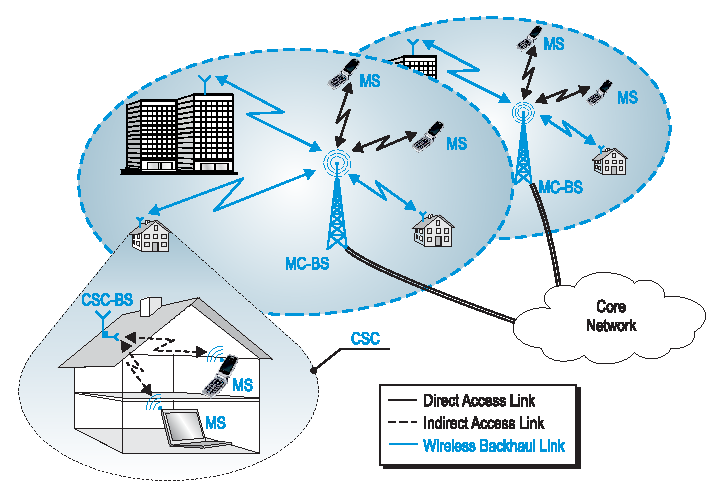
\includegraphics[width = \columnwidth]{figures/Cellular_Scenario_CR6F}
\caption{An illustration of the CSC deployment in a 5G network.}
\label{fig:scenario}
\end{figure}



Following the previous discussion, it is evident that spectrum extension and SCs are key-enablers for the 5G system.
%Recently, ElSawy \textit{et al.} \cite{Elsawy13} have presented Cognitive Small Cell (CSC), a concept that fulfills the capacity demands of the future wireless networks. 
Motivated by this fact, a preliminary concept of Cognitive Small Cell (CSC), a promising approach that jointly enhances the SC deployment and the efficient usage of the spectrum below \SI{6}{GHz} is presented. The notion of CSC has been previously investigated by Elsawy \textit{et al.} \cite{Elsawy13, Elsawy13_cmag}, where the authors primarily emphasized on the modelling techniques\footnote{The modelling is based on stochastic geometry, which allows a spatial averaging over multiple network geometries \cite{Haenggi, Haenggi08now}.} that depict the positioning of several CSCs inside the network. Due to this, the performance analysis of the CSC has been limited mainly to network abstraction. In contrast, this thesis emphasizes on key-aspects encountered while deploying a CSC, which otherwise could forbid its realization on a real hardware. %, which could possibly lead to a successful integration of CSCs in the 5G network. %Consequently, by considering different CR paradigms to enable secondary usage of the licensed spectrum, here a deeper comprehension of the concept is illustrated. %, thereby, making it accessible to 5G systems. 
%To strengthen our understanding of CSC, we demonstrate the feasibility of the respective paradigms by means of hardware implementations.
%Pertaining to the deployment, we analyze the true performance of the CSC as a CR application for the mentioned paradigms.  
 A comprehensive incorporation of CSC in a preliminary 5G architecture is illustrated in \figurename~\ref{fig:scenario}. In order to enhance the plausibility of the proposed network architecture, it is interesting to highlight some of the essential ingredients pertaining to the deployment of the CSC.

\subsubsection*{Network Elements}
 The following key elements are essential: a CSC-Base Station (CSC-BS), a Macro Cell-Base Station (MC-BS) and Mobile Stations (MSs), cf. \figurename~\ref{fig:scenario}. MSs are the devices either served by the MC-BS over a \textit{direct access} link or the CSC-BS over an \textit{indirect access} link. The direct access and the indirect access are the nomenclature used to distinguish a start-of-the-art access between the MC-BS and the MS from an access between the CSC-BS and the MS that represents a CR communication, respectively. Furthermore, the MC-BS is connected to several CSC-BSs over a \textit{wireless backhaul} link. Although the MC-BS and the MS already exist in the conventional cellular architecture, to incorporate the opportunistic access inside the CSC, it is necessary to consider a functionality upgrade.

\subsubsection*{Spectrum Access}
In the proposed network architecture, the access to the spectrum is realized over the wireless backhaul, the direct access and the indirect access links, cf. \figurename~\ref{fig:scenario}.
\begin{enumerate}
\item A wireless backhaul is a
%quasi-line of sight\footnote{It allows limited number of objects between the direct link.} 
point-to-point wireless link between the CSC-BS and MC-BS that relays the traffic generated from the CSC to the core network. Accounting the feasibility of ultra-dense CSC, the wireless backhaul link presents a cost-effective and energy-efficient alternative to the mobile operator.
With the limited infrastructure required for deployment, it accelerates installation and promotes scalability of the network.
For the wireless backhaul link, an exclusive spectrum for a longer duration is desired, hence, it is sensible to nominate a mmW band; alternatively, an exclusive band below \SI{6}{GHz} can be acquired using the principles of Licensed Shared Access \cite{ETSI13}.
%These WB links encourage ultra-densification as they brings down the capital expenditure and offer scalability to the vendor. 

\item A direct access link represents a direct access of the MS at the MC-BS over the allocated spectrum. Consequently, the spectrum access for this link is analogous to the one existing in the state-of-art wireless standards.
\item The CSC elements (the CSC-BS and the MS) are responsible for executing secondary access to the licensed spectrum. The additional spectrum acquired is used for the communication between the CSC-BS and the MS over the indirect access link.
\end{enumerate}

\subsubsection*{Network Compatibility}
Besides secondary access, CSC has to co-exist harmoniously with the other elements existing in the network. In this context, the network elements are embedded with additional functionality such as:
\begin{itemize}
\item The MS procures the control information (signalling and synchronization) over the indirect access link after connecting to the near-by CSC-BS.
\item In order to accomplish a logical placement of CSCs inside the network, the CSC employs S1 and X2 interfaces over the wireless backhaul link.
%Under this situation, the MC-BS, however, remains transparent to the additional spectrum acquired by the CSC over the IA link. 
%For the co-exisitence it is necessary to consider the co-existence of CSCs under the MC. 
\item For situations where several CSC-BSs co-exist under a MC-BS, operations like seamless cross-tier and co-tier mobility constitute a challenging task for the network.
\end{itemize}


\subsubsection*{Hardware Feasibility}
Along with other ingredients, it is essential to outline certain aspects that pertain to the hardware realizability of the CSC. For the CSC-BS, an antenna mount system consisting of an indoor and outdoor antenna is proposed. Whereby, the indoor antenna exploits the walls of the building to physically separate the indoor transmissions over the indirect access link, in this way, it curtails the interference to the primary system and neighbouring CSCs. Whereas, the outdoor antenna secures a narrow beam transmission to enhance the link quality for the wireless backhaul link. It is a well-known fact that Software Defined Radio (SDR) has played an important role in the genesis of the CR \cite{Jondral05}. In other words, in context with the CR, the SDR provides a suitable platform to approach rapid prototyping. Taking this into account, the SDR presents a viable solution for realizing (or demonstrating) the cognitive functionality pursued by the CSC-BS on a real hardware.


\subsubsection*{Indoor Deployment}
From the market analysis, it has been depicted that $70\%$ of the mobile traffic is originated indoor \cite{Chander08}. In addition, a new range of wireless services, categorized as Internet of Things, will operate from indoor. Thus, the effects will be far more consequential if we manage to consolidate these sources of traffic by means of SCs deployment. Hence, it is sensible to consider the residential and enterprise as the main deployment scenarios for the CSC, cf. \figurename~\ref{fig:scenario}. Except for a different coverage regime, the operating principles of these scenarios are analogous. Besides, in context with the CR, where the interference mitigation between the primary and secondary systems is a significant aspect, exercising the CR communication within the walls (which attributes to an indoor deployment) provides a spatial separation between the two systems. This, however, does not signifies that CR communications are only feasible for indoor scenarios. As the matter of fact, the indoor deployment is a technique for exploiting the behavioral dimension of the traffic source for a CR communication so that co-existence with the licensed users is facilitated. 
Based on this knowledge, an indoor scenario is considered for the deployment of the CSC, cf. \figurename~\ref{fig:scenario}.  

\subsection{Performance Analysis}
Since the evolution of wireless systems, understanding the performance of novel algorithms/techniques related to the wireless systems has always been a challenging task for the community. With regard to this, for a CR system, because of the involvement of two different systems namely primary and secondary systems, this task becomes even more difficult. On one side, it has been engaging a large number of researchers that are eager to find solutions for the new set of problems, leading them to develop theoretical models. %However, with the lack of concrete guidelines, different perspective have forward for the performance analysis.
 On the other side, due to the co-existence of the two systems sharing the same spectrum, the performance has been critical issue for the regulatory bodies and the mobile operators\footnote{For those operators who are willing to share their license (as primary system) and for those who are willing to access the licensed spectrum (as secondary system).}. With a multitude of theoretical models available in the literature, they are more attracted towards complete solutions and prefer to judge the performance of a CR based on hardware implementations. Due the different mindset across the two communities and the lack of concrete guidelines, there    
\section{Main Contributions}

\section{Organization}
